% Options for packages loaded elsewhere
\PassOptionsToPackage{unicode}{hyperref}
\PassOptionsToPackage{hyphens}{url}
%
\documentclass[
]{book}
\usepackage{lmodern}
\usepackage{amsmath}
\usepackage{ifxetex,ifluatex}
\ifnum 0\ifxetex 1\fi\ifluatex 1\fi=0 % if pdftex
  \usepackage[T1]{fontenc}
  \usepackage[utf8]{inputenc}
  \usepackage{textcomp} % provide euro and other symbols
  \usepackage{amssymb}
\else % if luatex or xetex
  \usepackage{unicode-math}
  \defaultfontfeatures{Scale=MatchLowercase}
  \defaultfontfeatures[\rmfamily]{Ligatures=TeX,Scale=1}
\fi
% Use upquote if available, for straight quotes in verbatim environments
\IfFileExists{upquote.sty}{\usepackage{upquote}}{}
\IfFileExists{microtype.sty}{% use microtype if available
  \usepackage[]{microtype}
  \UseMicrotypeSet[protrusion]{basicmath} % disable protrusion for tt fonts
}{}
\makeatletter
\@ifundefined{KOMAClassName}{% if non-KOMA class
  \IfFileExists{parskip.sty}{%
    \usepackage{parskip}
  }{% else
    \setlength{\parindent}{0pt}
    \setlength{\parskip}{6pt plus 2pt minus 1pt}}
}{% if KOMA class
  \KOMAoptions{parskip=half}}
\makeatother
\usepackage{xcolor}
\IfFileExists{xurl.sty}{\usepackage{xurl}}{} % add URL line breaks if available
\IfFileExists{bookmark.sty}{\usepackage{bookmark}}{\usepackage{hyperref}}
\hypersetup{
  pdftitle={REPORTS MADE EASY},
  pdfauthor={DIR-TERRANCE},
  hidelinks,
  pdfcreator={LaTeX via pandoc}}
\urlstyle{same} % disable monospaced font for URLs
\usepackage{color}
\usepackage{fancyvrb}
\newcommand{\VerbBar}{|}
\newcommand{\VERB}{\Verb[commandchars=\\\{\}]}
\DefineVerbatimEnvironment{Highlighting}{Verbatim}{commandchars=\\\{\}}
% Add ',fontsize=\small' for more characters per line
\usepackage{framed}
\definecolor{shadecolor}{RGB}{248,248,248}
\newenvironment{Shaded}{\begin{snugshade}}{\end{snugshade}}
\newcommand{\AlertTok}[1]{\textcolor[rgb]{0.94,0.16,0.16}{#1}}
\newcommand{\AnnotationTok}[1]{\textcolor[rgb]{0.56,0.35,0.01}{\textbf{\textit{#1}}}}
\newcommand{\AttributeTok}[1]{\textcolor[rgb]{0.77,0.63,0.00}{#1}}
\newcommand{\BaseNTok}[1]{\textcolor[rgb]{0.00,0.00,0.81}{#1}}
\newcommand{\BuiltInTok}[1]{#1}
\newcommand{\CharTok}[1]{\textcolor[rgb]{0.31,0.60,0.02}{#1}}
\newcommand{\CommentTok}[1]{\textcolor[rgb]{0.56,0.35,0.01}{\textit{#1}}}
\newcommand{\CommentVarTok}[1]{\textcolor[rgb]{0.56,0.35,0.01}{\textbf{\textit{#1}}}}
\newcommand{\ConstantTok}[1]{\textcolor[rgb]{0.00,0.00,0.00}{#1}}
\newcommand{\ControlFlowTok}[1]{\textcolor[rgb]{0.13,0.29,0.53}{\textbf{#1}}}
\newcommand{\DataTypeTok}[1]{\textcolor[rgb]{0.13,0.29,0.53}{#1}}
\newcommand{\DecValTok}[1]{\textcolor[rgb]{0.00,0.00,0.81}{#1}}
\newcommand{\DocumentationTok}[1]{\textcolor[rgb]{0.56,0.35,0.01}{\textbf{\textit{#1}}}}
\newcommand{\ErrorTok}[1]{\textcolor[rgb]{0.64,0.00,0.00}{\textbf{#1}}}
\newcommand{\ExtensionTok}[1]{#1}
\newcommand{\FloatTok}[1]{\textcolor[rgb]{0.00,0.00,0.81}{#1}}
\newcommand{\FunctionTok}[1]{\textcolor[rgb]{0.00,0.00,0.00}{#1}}
\newcommand{\ImportTok}[1]{#1}
\newcommand{\InformationTok}[1]{\textcolor[rgb]{0.56,0.35,0.01}{\textbf{\textit{#1}}}}
\newcommand{\KeywordTok}[1]{\textcolor[rgb]{0.13,0.29,0.53}{\textbf{#1}}}
\newcommand{\NormalTok}[1]{#1}
\newcommand{\OperatorTok}[1]{\textcolor[rgb]{0.81,0.36,0.00}{\textbf{#1}}}
\newcommand{\OtherTok}[1]{\textcolor[rgb]{0.56,0.35,0.01}{#1}}
\newcommand{\PreprocessorTok}[1]{\textcolor[rgb]{0.56,0.35,0.01}{\textit{#1}}}
\newcommand{\RegionMarkerTok}[1]{#1}
\newcommand{\SpecialCharTok}[1]{\textcolor[rgb]{0.00,0.00,0.00}{#1}}
\newcommand{\SpecialStringTok}[1]{\textcolor[rgb]{0.31,0.60,0.02}{#1}}
\newcommand{\StringTok}[1]{\textcolor[rgb]{0.31,0.60,0.02}{#1}}
\newcommand{\VariableTok}[1]{\textcolor[rgb]{0.00,0.00,0.00}{#1}}
\newcommand{\VerbatimStringTok}[1]{\textcolor[rgb]{0.31,0.60,0.02}{#1}}
\newcommand{\WarningTok}[1]{\textcolor[rgb]{0.56,0.35,0.01}{\textbf{\textit{#1}}}}
\usepackage{longtable,booktabs}
\usepackage{calc} % for calculating minipage widths
% Correct order of tables after \paragraph or \subparagraph
\usepackage{etoolbox}
\makeatletter
\patchcmd\longtable{\par}{\if@noskipsec\mbox{}\fi\par}{}{}
\makeatother
% Allow footnotes in longtable head/foot
\IfFileExists{footnotehyper.sty}{\usepackage{footnotehyper}}{\usepackage{footnote}}
\makesavenoteenv{longtable}
\usepackage{graphicx}
\makeatletter
\def\maxwidth{\ifdim\Gin@nat@width>\linewidth\linewidth\else\Gin@nat@width\fi}
\def\maxheight{\ifdim\Gin@nat@height>\textheight\textheight\else\Gin@nat@height\fi}
\makeatother
% Scale images if necessary, so that they will not overflow the page
% margins by default, and it is still possible to overwrite the defaults
% using explicit options in \includegraphics[width, height, ...]{}
\setkeys{Gin}{width=\maxwidth,height=\maxheight,keepaspectratio}
% Set default figure placement to htbp
\makeatletter
\def\fps@figure{htbp}
\makeatother
\setlength{\emergencystretch}{3em} % prevent overfull lines
\providecommand{\tightlist}{%
  \setlength{\itemsep}{0pt}\setlength{\parskip}{0pt}}
\setcounter{secnumdepth}{5}
\usepackage{booktabs}
\ifluatex
  \usepackage{selnolig}  % disable illegal ligatures
\fi
\usepackage[]{natbib}
\bibliographystyle{apalike}

\title{REPORTS MADE EASY}
\author{DIR-TERRANCE\footnote{FOUNDER:RWILLS STATISTICAL COMPANY,EMAIL:\href{mailto:consultancyrwillsstats@gmail.com}{\nolinkurl{consultancyrwillsstats@gmail.com}}}}
\date{2021-02-08}

\begin{document}
\maketitle

{
\setcounter{tocdepth}{1}
\tableofcontents
}
\hypertarget{prerequisites}{%
\chapter*{Prerequisites}\label{prerequisites}}
\addcontentsline{toc}{chapter}{Prerequisites}

\hypertarget{packages.}{%
\section{Packages.}\label{packages.}}

Install the following packages to follow the book easily.

\begin{Shaded}
\begin{Highlighting}[]
\CommentTok{\#install.packages("bookdown") \#to generate the book.}
\DocumentationTok{\#\# or the development version}
\DocumentationTok{\#\# devtools::install\_github("rstudio/bookdown")}
\CommentTok{\# }
\CommentTok{\#install.packages("tidyverse")\# a collection of r packages that makes working with data easier.}

\FunctionTok{library}\NormalTok{(tidyverse)}
\end{Highlighting}
\end{Shaded}

\begin{verbatim}
## -- Attaching packages --------------------------------------- tidyverse 1.3.0 --
\end{verbatim}

\begin{verbatim}
## v ggplot2 3.3.3     v purrr   0.3.4
## v tibble  3.0.6     v dplyr   1.0.4
## v tidyr   1.1.2     v stringr 1.4.0
## v readr   1.4.0     v forcats 0.5.1
\end{verbatim}

\begin{verbatim}
## -- Conflicts ------------------------------------------ tidyverse_conflicts() --
## x dplyr::filter() masks stats::filter()
## x dplyr::lag()    masks stats::lag()
\end{verbatim}

\begin{Shaded}
\begin{Highlighting}[]
\CommentTok{\#}

\CommentTok{\#install.packages("rticles")\# journal like template}

\FunctionTok{library}\NormalTok{(rticles)}
\CommentTok{\#}
\CommentTok{\#install.packages()}
\CommentTok{\#}
\FunctionTok{library}\NormalTok{(data.table)}
\end{Highlighting}
\end{Shaded}

\begin{verbatim}
## 
## Attaching package: 'data.table'
\end{verbatim}

\begin{verbatim}
## The following objects are masked from 'package:dplyr':
## 
##     between, first, last
\end{verbatim}

\begin{verbatim}
## The following object is masked from 'package:purrr':
## 
##     transpose
\end{verbatim}

\begin{Shaded}
\begin{Highlighting}[]
\FunctionTok{library}\NormalTok{(RColorBrewer)}
\end{Highlighting}
\end{Shaded}

\hypertarget{bibliography}{%
\subsection{Bibliography}\label{bibliography}}

automatically create a bib database for R packages

\begin{Shaded}
\begin{Highlighting}[]
\NormalTok{knitr}\SpecialCharTok{::}\FunctionTok{write\_bib}\NormalTok{(}\FunctionTok{c}\NormalTok{(}
  \FunctionTok{.packages}\NormalTok{(), }\StringTok{\textquotesingle{}bookdown\textquotesingle{}}\NormalTok{, }\StringTok{\textquotesingle{}knitr\textquotesingle{}}\NormalTok{, }\StringTok{\textquotesingle{}rmarkdown\textquotesingle{}}\NormalTok{, }\StringTok{\textquotesingle{}tidyverse\textquotesingle{}}
\NormalTok{), }\StringTok{\textquotesingle{}packages.bib\textquotesingle{}}\NormalTok{)}
\end{Highlighting}
\end{Shaded}

\hypertarget{intro}{%
\chapter{Introduction}\label{intro}}

\hypertarget{challenger}{%
\section{THE CHALLLENGER.}\label{challenger}}

If you have ever been in a data analytics class I bet you have ever heard of \href{https://www.tufte.com}{Edward Tufte}. On his critisim on the engineers' failures to make sense of the concerns the had on lunching \href{https://www.nasa/challenger/.com}{The Challenger} on January 28, 1986.

\begin{quote}
Being Right isn't enough, you have to be convincing.

\textasciitilde{} Edward Tufte
\end{quote}

This philosophy formed the basis of his arguments in his book \emph{Visual Explanations and Quantities, Evidence and Narrative}

\begin{quote}
An essential analytic task in making decisions based on evidence
is to understand how things work---mechanism, trade-offs, process
and dynamics, cause and effect. That is, intervention-thinking and
policy-thinking demand causality-thinking
\end{quote}

\begin{quote}
Making decisions based on evidence requires the appropriate display
of that evidence. Good displays of data help to reveal knowledge
relevant to understanding mechanism, process and dynamics, cause
and effect. That is, displays of statistical data should directly serve the
analytic task at hand.
\end{quote}

Hence we are going set our reports right even before we begin in whatever we are supposed to report on.

\hypertarget{data}{%
\section{DATA}\label{data}}

Lets take an hypothetical data where in Africa the distance students take to walk to get access to basic education affect their perfomance.

\begin{Shaded}
\begin{Highlighting}[]
\FunctionTok{set.seed}\NormalTok{(}\DecValTok{123}\NormalTok{)}
\NormalTok{n }\OtherTok{\textless{}{-}} \DecValTok{30}
\NormalTok{df }\OtherTok{\textless{}{-}} \FunctionTok{tibble}\NormalTok{(}
  \AttributeTok{score=}\FunctionTok{sample}\NormalTok{(}\DecValTok{30}\SpecialCharTok{:}\DecValTok{99}\NormalTok{, }\AttributeTok{size =}\NormalTok{ n, }\AttributeTok{replace =}\NormalTok{ T),}
  \AttributeTok{dist=}\FunctionTok{sample}\NormalTok{(}\DecValTok{1}\SpecialCharTok{:}\DecValTok{8}\NormalTok{, }\AttributeTok{size=}\NormalTok{n, }\AttributeTok{replace =}\NormalTok{ T)}
\NormalTok{)}

\FunctionTok{head}\NormalTok{(df)}\CommentTok{\#Checking the first six observations}
\end{Highlighting}
\end{Shaded}

\begin{verbatim}
## # A tibble: 6 x 2
##   score  dist
##   <int> <int>
## 1    60     8
## 2    80     6
## 3    43     1
## 4    96     2
## 5    71     5
## 6    79     5
\end{verbatim}

\begin{Shaded}
\begin{Highlighting}[]
\DocumentationTok{\#\#\# Any time you get data into your hands always check its health status ie, the first thing you get in a hospital is checking weight, height, BMI, blood pressure etc.}
\DocumentationTok{\#\#\# }
\DocumentationTok{\#\#\# Height \& Weight}
\FunctionTok{nrow}\NormalTok{(df)}\CommentTok{\#number of rows}
\end{Highlighting}
\end{Shaded}

\begin{verbatim}
## [1] 30
\end{verbatim}

\begin{Shaded}
\begin{Highlighting}[]
\FunctionTok{ncol}\NormalTok{(df)}\CommentTok{\#number of columns}
\end{Highlighting}
\end{Shaded}

\begin{verbatim}
## [1] 2
\end{verbatim}

\begin{Shaded}
\begin{Highlighting}[]
\DocumentationTok{\#\#\# Pressure}
\FunctionTok{str}\NormalTok{(df)}\CommentTok{\#structure}
\end{Highlighting}
\end{Shaded}

\begin{verbatim}
## tibble [30 x 2] (S3: tbl_df/tbl/data.frame)
##  $ score: int [1:30] 60 80 43 96 71 79 72 43 54 98 ...
##  $ dist : int [1:30] 8 6 1 2 5 5 8 4 7 5 ...
\end{verbatim}

\begin{Shaded}
\begin{Highlighting}[]
\DocumentationTok{\#\#\# BMI}
\FunctionTok{dim}\NormalTok{(df) }
\end{Highlighting}
\end{Shaded}

\begin{verbatim}
## [1] 30  2
\end{verbatim}

\begin{Shaded}
\begin{Highlighting}[]
\FunctionTok{colnames}\NormalTok{(df)}
\end{Highlighting}
\end{Shaded}

\begin{verbatim}
## [1] "score" "dist"
\end{verbatim}

\begin{Shaded}
\begin{Highlighting}[]
\DocumentationTok{\#\#\# }
\end{Highlighting}
\end{Shaded}

You can label chapter and section titles using \texttt{\{\#label\}} after them, e.g., we can reference Chapter \ref{intro}. If you do not manually label them, there will be automatic labels anyway, e.g., Chapter \ref{methods}.

Figures and tables with captions will be placed in \texttt{figure} and \texttt{table} environments, respectively.

\begin{Shaded}
\begin{Highlighting}[]
\FunctionTok{par}\NormalTok{(}\AttributeTok{mar =} \FunctionTok{c}\NormalTok{(}\DecValTok{4}\NormalTok{, }\DecValTok{4}\NormalTok{, .}\DecValTok{1}\NormalTok{, .}\DecValTok{1}\NormalTok{))}
\FunctionTok{plot}\NormalTok{(pressure, }\AttributeTok{type =} \StringTok{\textquotesingle{}b\textquotesingle{}}\NormalTok{, }\AttributeTok{pch =} \DecValTok{19}\NormalTok{)}
\end{Highlighting}
\end{Shaded}

\begin{figure}

{\centering 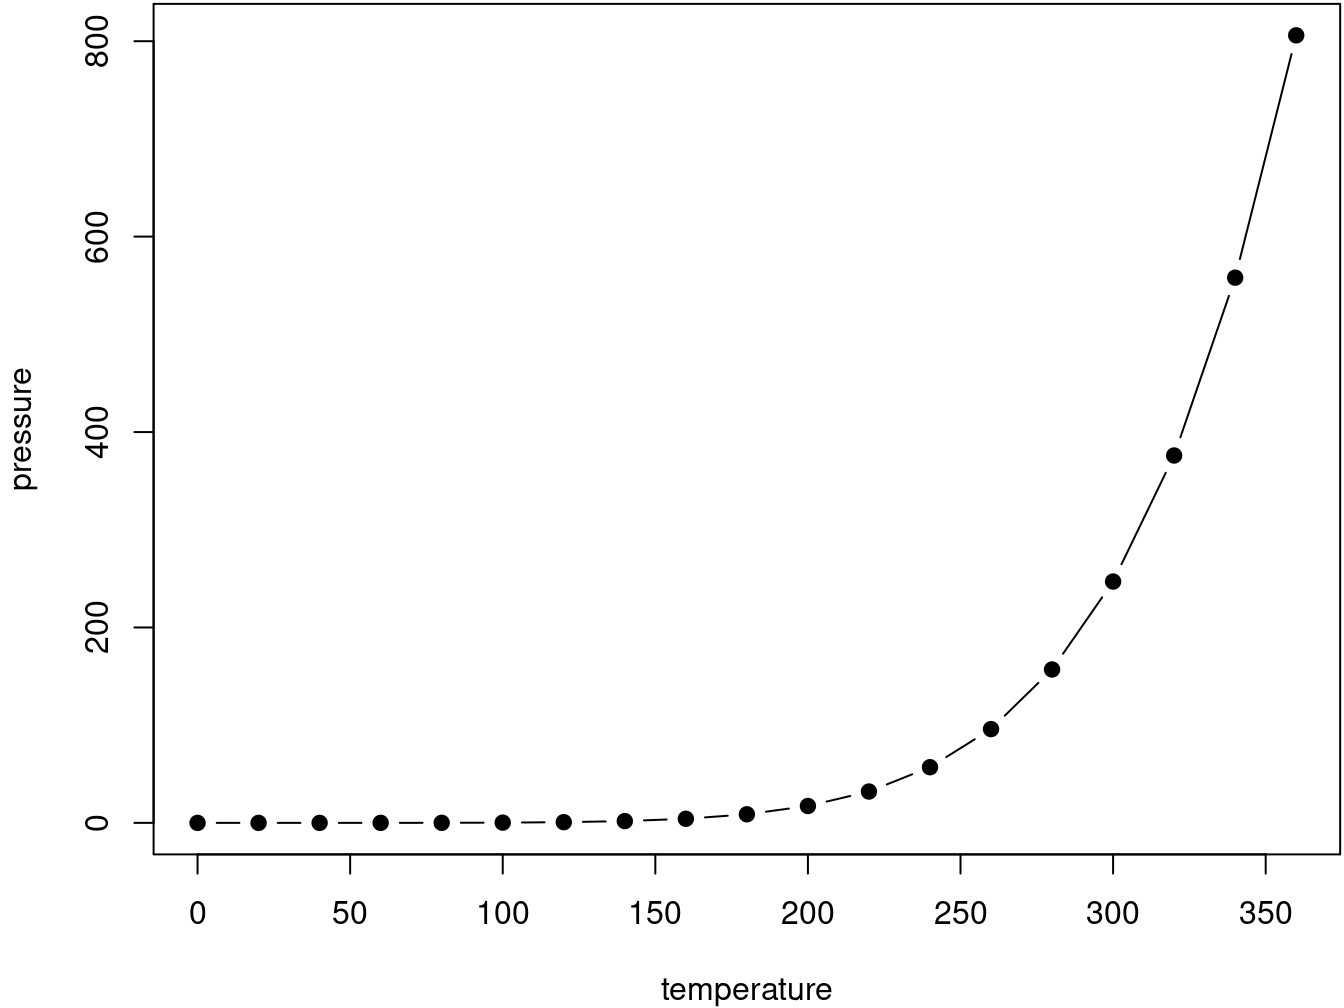
\includegraphics[width=0.8\linewidth]{REPORTS-MADE-EASY_files/figure-latex/nice-fig-1} 

}

\caption{Here is a nice figure!}\label{fig:nice-fig}
\end{figure}

Reference a figure by its code chunk label with the \texttt{fig:} prefix, e.g., see Figure \ref{fig:nice-fig}. Similarly, you can reference tables generated from \texttt{knitr::kable()}, e.g., see Table \ref{tab:nice-tab}.

\begin{Shaded}
\begin{Highlighting}[]
\NormalTok{knitr}\SpecialCharTok{::}\FunctionTok{kable}\NormalTok{(}
  \FunctionTok{head}\NormalTok{(iris, }\DecValTok{20}\NormalTok{), }\AttributeTok{caption =} \StringTok{\textquotesingle{}Here is a nice table!\textquotesingle{}}\NormalTok{,}
  \AttributeTok{booktabs =} \ConstantTok{TRUE}
\NormalTok{)}
\end{Highlighting}
\end{Shaded}

\begin{table}

\caption{\label{tab:nice-tab}Here is a nice table!}
\centering
\begin{tabular}[t]{rrrrl}
\toprule
Sepal.Length & Sepal.Width & Petal.Length & Petal.Width & Species\\
\midrule
5.1 & 3.5 & 1.4 & 0.2 & setosa\\
4.9 & 3.0 & 1.4 & 0.2 & setosa\\
4.7 & 3.2 & 1.3 & 0.2 & setosa\\
4.6 & 3.1 & 1.5 & 0.2 & setosa\\
5.0 & 3.6 & 1.4 & 0.2 & setosa\\
\addlinespace
5.4 & 3.9 & 1.7 & 0.4 & setosa\\
4.6 & 3.4 & 1.4 & 0.3 & setosa\\
5.0 & 3.4 & 1.5 & 0.2 & setosa\\
4.4 & 2.9 & 1.4 & 0.2 & setosa\\
4.9 & 3.1 & 1.5 & 0.1 & setosa\\
\addlinespace
5.4 & 3.7 & 1.5 & 0.2 & setosa\\
4.8 & 3.4 & 1.6 & 0.2 & setosa\\
4.8 & 3.0 & 1.4 & 0.1 & setosa\\
4.3 & 3.0 & 1.1 & 0.1 & setosa\\
5.8 & 4.0 & 1.2 & 0.2 & setosa\\
\addlinespace
5.7 & 4.4 & 1.5 & 0.4 & setosa\\
5.4 & 3.9 & 1.3 & 0.4 & setosa\\
5.1 & 3.5 & 1.4 & 0.3 & setosa\\
5.7 & 3.8 & 1.7 & 0.3 & setosa\\
5.1 & 3.8 & 1.5 & 0.3 & setosa\\
\bottomrule
\end{tabular}
\end{table}

You can write citations, too. For example, we are using the \textbf{bookdown} package \citep{R-bookdown} in this sample book, which was built on top of R Markdown and \textbf{knitr} \citep{xie2015}.

\hypertarget{eda}{%
\chapter{EXPLANATORY DATA ANALYSIS}\label{eda}}

Here we form the foundation of our report. We listen to what the data has for us.This should be the entry step in a data project, where we start by knowing the correct data types and exploring distributions in numerical and categorical variables.
Always getting your data into the right format will affect how you work with them hence inferences that they generate.

At this point we perfom dataset \emph{`anatomy'} namely;

\begin{verbatim}
    *Getting metrics like total rows, columns, data types, zeros, and missing values
    *How each of the previous items impacts on different analysis
    *How to quickly filter and select variables.
    
    *Univariate analysis in categorical variable:
       
       +Frequency, percentage, cumulative value, and colorful plots
    *Univariate analysis with numerical variables:
       +Percentile, dispersion, standard deviation, mean, top and bottom values
      +Plotting distributions
\end{verbatim}

Based on our \ref{data} we can develop the following questions.

\begin{verbatim}
*Can we divide the perfomance into fail and passed?
*What distance community does one above categories fall into?
\end{verbatim}

\hypertarget{dw}{%
\section{DATA WRANGLING}\label{dw}}

\begin{Shaded}
\begin{Highlighting}[]
\NormalTok{df}\SpecialCharTok{$}\NormalTok{performance }\OtherTok{\textless{}{-}} \FunctionTok{fifelse}\NormalTok{(df}\SpecialCharTok{$}\NormalTok{score}\SpecialCharTok{\textgreater{}=}\DecValTok{40}\NormalTok{, }\AttributeTok{yes =} \StringTok{"passed"}\NormalTok{, }\AttributeTok{no=}\StringTok{"failed"}\NormalTok{) }\CommentTok{\#answering the first question.}
\NormalTok{df}\SpecialCharTok{$}\NormalTok{dist\_comm }\OtherTok{\textless{}{-}} \FunctionTok{fifelse}\NormalTok{(df}\SpecialCharTok{$}\NormalTok{dist}\SpecialCharTok{\textless{}=}\DecValTok{1}\NormalTok{, }\AttributeTok{yes =} \StringTok{"near"}\NormalTok{,}
                        \FunctionTok{fifelse}\NormalTok{(df}\SpecialCharTok{$}\NormalTok{dist}\SpecialCharTok{\textgreater{}}\DecValTok{1} \SpecialCharTok{\&}\NormalTok{ df}\SpecialCharTok{$}\NormalTok{dist}\SpecialCharTok{\textless{}=}\DecValTok{4}\NormalTok{,}
                                \AttributeTok{yes=}\StringTok{"average"}\NormalTok{,}
                                \AttributeTok{no=}\StringTok{"far"}\NormalTok{)}
\NormalTok{                        )}\CommentTok{\#answering the second question.}
\NormalTok{df}\SpecialCharTok{$}\NormalTok{dist }\OtherTok{\textless{}{-}} \FunctionTok{as.factor}\NormalTok{(df}\SpecialCharTok{$}\NormalTok{dist)}
\NormalTok{df}\SpecialCharTok{$}\NormalTok{dist\_comm }\OtherTok{\textless{}{-}} \FunctionTok{as.factor}\NormalTok{(df}\SpecialCharTok{$}\NormalTok{dist\_comm)}
\NormalTok{df}\SpecialCharTok{$}\NormalTok{performance }\OtherTok{\textless{}{-}} \FunctionTok{as.factor}\NormalTok{(df}\SpecialCharTok{$}\NormalTok{performance)}
\end{Highlighting}
\end{Shaded}

\hypertarget{vis}{%
\section{Visualization}\label{vis}}

\begin{Shaded}
\begin{Highlighting}[]
\NormalTok{df }\SpecialCharTok{\%\textgreater{}\%} 
  \FunctionTok{ggplot}\NormalTok{(}\FunctionTok{aes}\NormalTok{(dist, score))}\SpecialCharTok{+}
  \FunctionTok{geom\_boxplot}\NormalTok{()}\SpecialCharTok{+}
  \FunctionTok{labs}\NormalTok{(}\AttributeTok{title =} \StringTok{"BOXPLOT OF STUDENTS\textquotesingle{}}\SpecialCharTok{\textbackslash{}n}\StringTok{SCORE BASED ON DISTANCE."}\NormalTok{)}
\end{Highlighting}
\end{Shaded}

\begin{figure}

{\centering 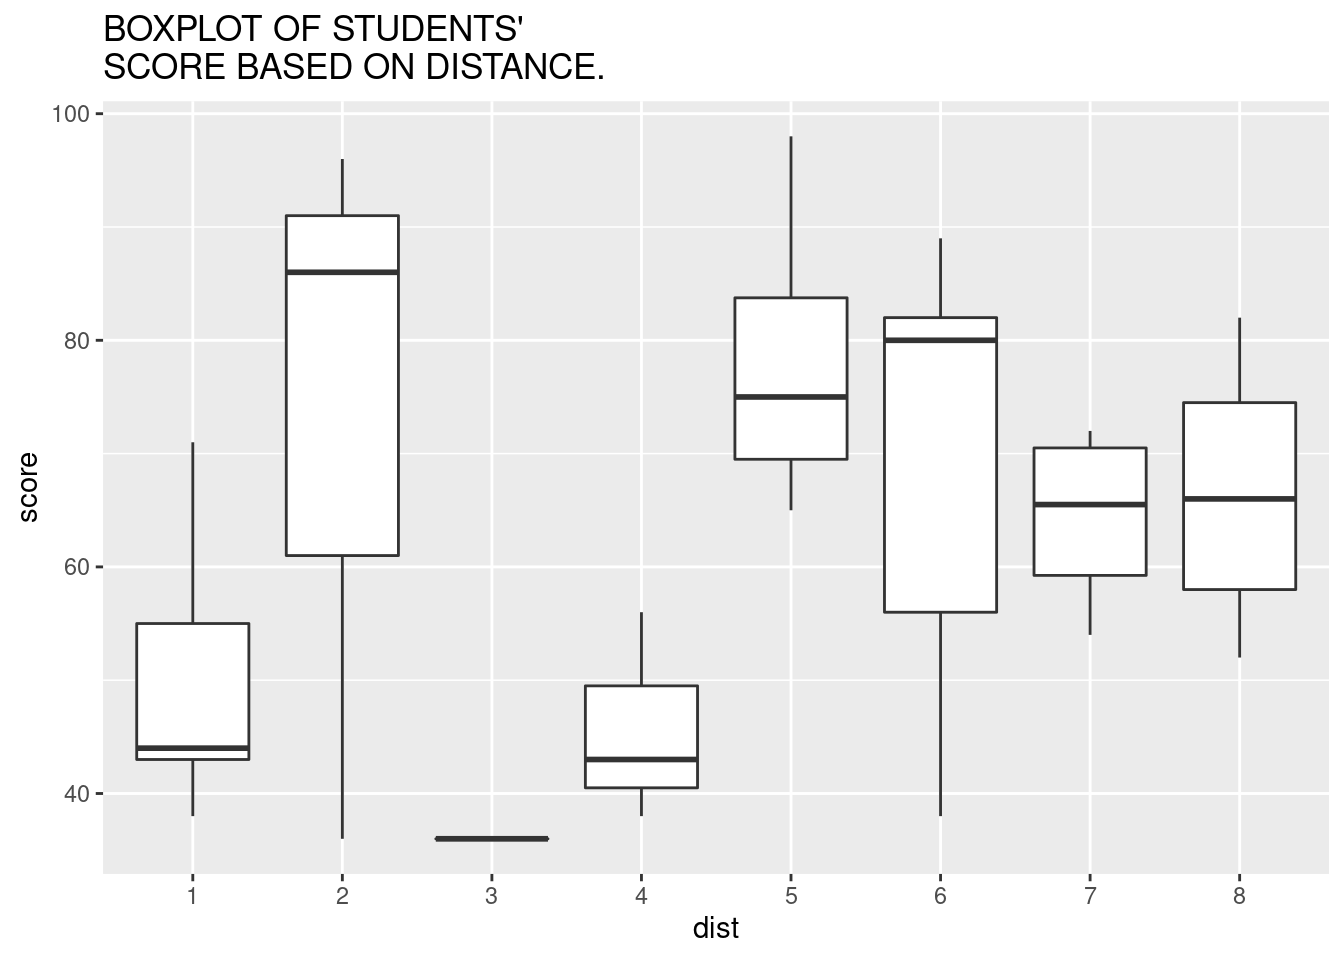
\includegraphics[width=0.8\linewidth]{REPORTS-MADE-EASY_files/figure-latex/visBox-fig-1} 

}

\caption{boxplot of score based pn distance students walk}\label{fig:visBox-fig}
\end{figure}

Its results above is astonishing, for see students in coming from distance 3-4 perform even better than those who are close to school.

\begin{Shaded}
\begin{Highlighting}[]
\NormalTok{df }\SpecialCharTok{\%\textgreater{}\%} 
  \FunctionTok{ggplot}\NormalTok{(}\FunctionTok{aes}\NormalTok{(}\AttributeTok{y=}\NormalTok{score, }\AttributeTok{fill=}\NormalTok{performance))}\SpecialCharTok{+}
  \FunctionTok{geom\_bar}\NormalTok{(}\AttributeTok{position =} \StringTok{"stack"}\NormalTok{)}\SpecialCharTok{+}
  \FunctionTok{facet\_wrap}\NormalTok{(}\SpecialCharTok{\textasciitilde{}}\NormalTok{performance)}\SpecialCharTok{+}
  \FunctionTok{labs}\NormalTok{(}\AttributeTok{title =} \StringTok{"Bargraph OF STUDENTS\textquotesingle{}}\SpecialCharTok{\textbackslash{}n}\StringTok{SCORE."}\NormalTok{)}
\end{Highlighting}
\end{Shaded}

\begin{figure}

{\centering 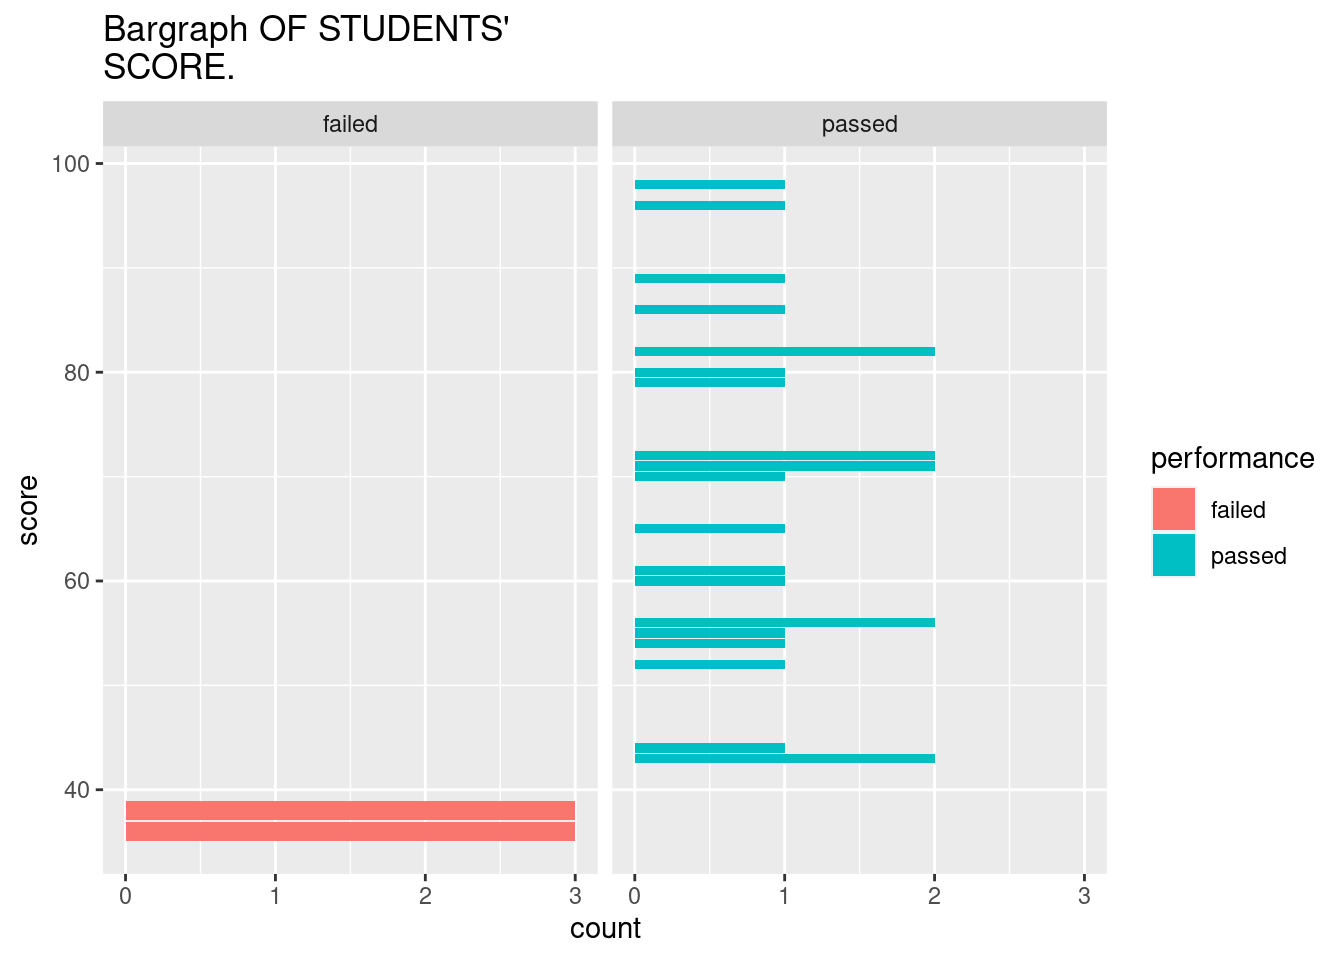
\includegraphics{REPORTS-MADE-EASY_files/figure-latex/visBar-fig-1} 

}

\caption{Bargraphs}\label{fig:visBar-fig-1}
\end{figure}

\begin{Shaded}
\begin{Highlighting}[]
\NormalTok{df }\SpecialCharTok{\%\textgreater{}\%} 
  \FunctionTok{ggplot}\NormalTok{(}\FunctionTok{aes}\NormalTok{(}\AttributeTok{y=}\NormalTok{score, }\AttributeTok{fill=}\NormalTok{performance))}\SpecialCharTok{+}
  \FunctionTok{geom\_bar}\NormalTok{(}\AttributeTok{position =} \StringTok{"identity"}\NormalTok{)}\SpecialCharTok{+}
  \FunctionTok{facet\_wrap}\NormalTok{(}\SpecialCharTok{\textasciitilde{}}\NormalTok{dist\_comm)}\SpecialCharTok{+}
  \FunctionTok{labs}\NormalTok{(}\AttributeTok{title =} \StringTok{"Bargraph OF STUDENTS\textquotesingle{}}\SpecialCharTok{\textbackslash{}n}\StringTok{SCORE. IN DIFFERENT DISTANCE COMMUNITIES"}\NormalTok{)}
\end{Highlighting}
\end{Shaded}

\begin{figure}

{\centering 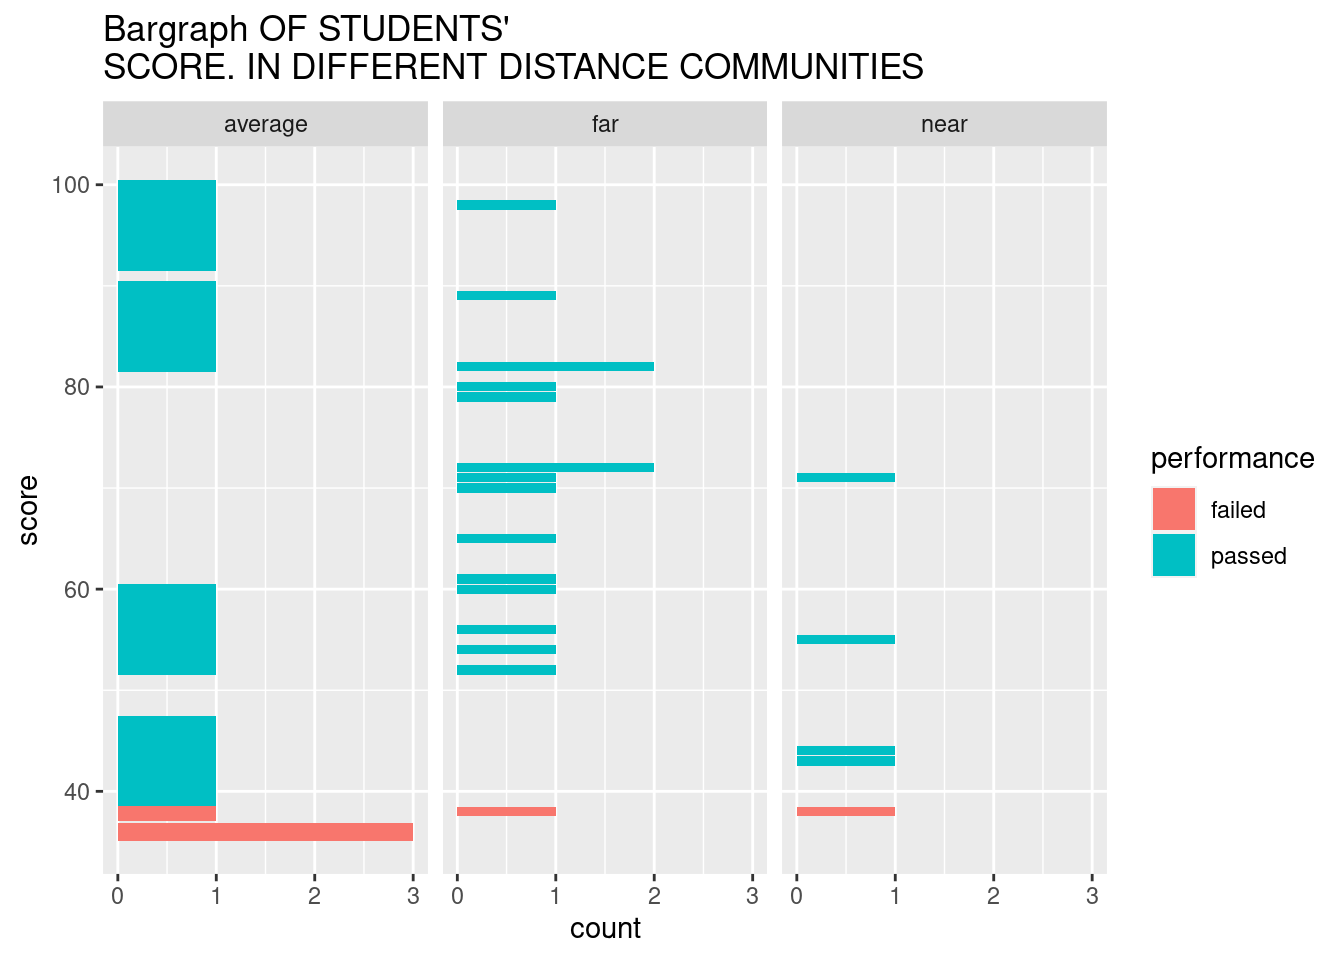
\includegraphics{REPORTS-MADE-EASY_files/figure-latex/visBar-fig-2} 

}

\caption{Bargraphs}\label{fig:visBar-fig-2}
\end{figure}

\hypertarget{mods}{%
\chapter{MODELS/METHODS}\label{mods}}

Now that we have seen some interesting patterns, lets try to get the finnier details of them.
Modeling is important for they reveal subtle stories in a data.

\begin{quote}
All models are wrong. Some models are useful.

\begin{verbatim}
                                          ~Author(Statistical Modelling)
\end{verbatim}
\end{quote}

\begin{quote}
Art is a lie that tells the truth!

\begin{verbatim}
                                                       ~Pablo Picasso
\end{verbatim}
\end{quote}

There are as many named lists of models as sand, yet they all have one thing in common;

\begin{quote}
A model is a representative of a specific purpose.
\end{quote}

Hence the appropriate form of the model depends on the task at hand and the expertise of the scientist.

\hypertarget{uses-of-statistical-modelsstatmods.}{%
\section[USES OF STATISTICAL MODELS\{\#statMods\}.]{\texorpdfstring{USES OF STATISTICAL MODELS\{\#statMods\}\footnote{There are several classification of models eg. Mathematical and Statistical models, how you define a model changes its classification hence affecting its application}.}{USES OF STATISTICAL MODELS\{\#statMods\}.}}\label{uses-of-statistical-modelsstatmods.}}

\begin{verbatim}
*Description models
*Classification or prediction models.
*Anticipating the consequences of interventions models.
\end{verbatim}

Its difficult to use observation to inform concrete knowledge becausse r/ships are complicated and involve multiple factors, do you still recall the mistakes made by the challengers' engineers?\ref{challenger}.

\begin{quote}
Mathematicians(``Statisticians'') do not study objects, butbthe relations among objetcs.

\begin{verbatim}
                                                         ~Georges Braque
\end{verbatim}
\end{quote}

Lets consider our case data \ref{dw}, we want to build a simple model that predicts a students performance based on the distance community(Sometimes variables will have collinearity hence be keen.)

\[
Y=\beta_0+\beta X +e
\]

\begin{Shaded}
\begin{Highlighting}[]
\NormalTok{mod }\OtherTok{\textless{}{-}} \FunctionTok{lm}\NormalTok{(}\AttributeTok{formula =}\NormalTok{score}\SpecialCharTok{\textasciitilde{}}\NormalTok{dist\_comm, }\AttributeTok{data =}\NormalTok{ df)}

\FunctionTok{anova}\NormalTok{(mod)}
\end{Highlighting}
\end{Shaded}

\begin{verbatim}
## Analysis of Variance Table
## 
## Response: score
##           Df Sum Sq Mean Sq F value  Pr(>F)  
## dist_comm  2 2240.1 1120.03  3.5759 0.04191 *
## Residuals 27 8456.9  313.22                  
## ---
## Signif. codes:  0 '***' 0.001 '**' 0.01 '*' 0.05 '.' 0.1 ' ' 1
\end{verbatim}

\begin{Shaded}
\begin{Highlighting}[]
\FunctionTok{summary}\NormalTok{(mod)}
\end{Highlighting}
\end{Shaded}

\begin{verbatim}
## 
## Call:
## lm(formula = score ~ dist_comm, data = df)
## 
## Residuals:
##     Min      1Q  Median      3Q     Max 
## -31.471 -13.153  -1.971  10.279  42.625 
## 
## Coefficients:
##               Estimate Std. Error t value Pr(>|t|)    
## (Intercept)     53.375      6.257   8.530 3.82e-09 ***
## dist_commfar    16.096      7.588   2.121   0.0432 *  
## dist_commnear   -3.175     10.089  -0.315   0.7554    
## ---
## Signif. codes:  0 '***' 0.001 '**' 0.01 '*' 0.05 '.' 0.1 ' ' 1
## 
## Residual standard error: 17.7 on 27 degrees of freedom
## Multiple R-squared:  0.2094, Adjusted R-squared:  0.1508 
## F-statistic: 3.576 on 2 and 27 DF,  p-value: 0.04191
\end{verbatim}

\hypertarget{remarks}{%
\chapter{REMARKS}\label{remarks}}

Awesome unlike the engineers you will never have to face the Tuftes' criticisms.

  \bibliography{book.bib,packages.bib}

\end{document}
